\documentclass{beamer}
\usepackage{amsmath, amssymb}
\usepackage{graphicx}
\usepackage[inline]{asymptote}
\usepackage{hyperref}

\title{Understanding Luck: A Mathematical Exploration}
\author{Warren D. MacEvoy}
\date{\today}

\begin{document}

\frame{\titlepage}

% Slide 1: Introduction
\begin{frame}
\frametitle{Introduction to Luck}
\begin{itemize}
    \item \textbf{What is Luck?}
        \begin{itemize}
            \item Luck quantifies how likely an outcome is compared to others.
            \item Formal definition: 
            \[L(x) = |\Omega(x)| + \frac{1}{2}|\omega(x)|\]
        \end{itemize}
    \item \textbf{Range of Luck:} 0 (unlucky) to 1 (very lucky), average luck is 0.5.
    \item \textbf{Why Study Luck?}
        \begin{itemize}
            \item Luck connects mathematical probability to real-world scenarios.
            \item Examples: Password guessing, random tennis ball tosses.
        \end{itemize}
\end{itemize}
\end{frame}

% Slide 2: Example: Luck in Coin Tosses
\begin{frame}
\frametitle{Example: Luck in Coin Tosses}
\begin{itemize}
    \item Consider 8 fair coin flips.
    \item What is the luck of getting exactly 4 heads?
    \[
    p(x) = \frac{8!}{4!(8-4)!} \left( \frac{1}{2} \right)^8
    \]
    \item Luck for different outcomes is computed using the binomial distribution.
    \item \textbf{Table:} Luck values for outcomes
    \begin{center}
    \begin{tabular}{|c|c|}
    \hline
    Number of Heads & Luck Value \\
    \hline
    0 or 8 & 0.996 \\
    1 or 7 & 0.961 \\
    2 or 6 & 0.820 \\
    3 or 5 & 0.492 \\
    4 & 0.136 \\
    \hline
    \end{tabular}
    \end{center}
\end{itemize}
\end{frame}

% Slide 3: Normal Distribution and Luck
\begin{frame}
\frametitle{Luck in the Normal Distribution}
\begin{itemize}
    \item Consider the 1D normal distribution with mean \(\mu\) and variance \(\sigma^2\):
    \[
    p(x) = \frac{1}{\sqrt{2\pi \sigma^2}} e^{-\frac{(x - \mu)^2}{2\sigma^2}}
    \]
    \item The luck of an outcome is:
    \[
    L(x) = \text{erf}\left(\frac{x - \mu}{\sqrt{2\sigma^2}}\right)
    \]
    \item Approximate formula for luck:
    \[
    L(x) \approx \frac{1}{2} \left[ 1 + \text{erf}\left( \frac{x - \mu}{\sqrt{\sigma^2}} - \sqrt{\frac{1}{2}} \right) \right]
    \]
    \item Exact vs Approximate Luck: Use of asymptotic formulas for large dimensions.
\end{itemize}
\end{frame}

% Slide 4: Visualizing Luck for Normal Distribution
\begin{frame}
\frametitle{Visualization: Luck in Normal Distribution}
\begin{center}
    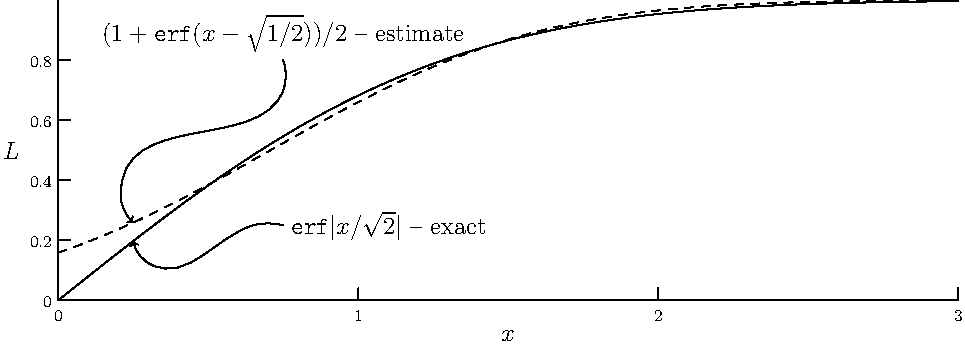
\includegraphics[width=0.8\textwidth]{graphics/normal1.pdf}
\end{center}
\end{frame}

% Slide 6: Z-Luck and its Applications
\begin{frame}
\frametitle{Z-Luck: Combining Luck from Experiments}
\begin{itemize}
    \item Z-luck allows us to combine results from multiple independent experiments.
    \item Formula for z-luck:
    \[
    z_L = \sqrt{\Sigma^{-1}(x - \mu)} - \sqrt{df - \frac{1}{2}}
    \]
    \item Example: Combining observations from normal distributions across different dimensions.
    \item Application in determining whether results from independent experiments align or not.
\end{itemize}
\end{frame}

% Slide 7: Application: Testing Randomness
\begin{frame}
\frametitle{Application: Testing Randomness}
\begin{itemize}
    \item Randomness tests like Dieharder use luck to validate random number generators.
    \item \textbf{Max64 Test:} Combines multiple independent tests to compute a luck score.
    \item Luck is used to distinguish between weak randomness and fully random outcomes.
    \item Inconsistent randomness leads to large or small z-luck values.
\end{itemize}
\end{frame}

% Slide 8: Conclusion
\begin{frame}
\frametitle{Conclusion}
\begin{itemize}
    \item Luck is a versatile concept connecting probability and real-world events.
    \item Applications range from testing randomness to real-world problem-solving.
    \item Key insights:
        \begin{itemize}
            \item Uniformity of luck across distributions.
            \item Elliptical shell behavior in multinomial distributions.
        \end{itemize}
    \item Thank you! Questions?
\end{itemize}
\end{frame}

\end{document}
